\documentclass{article}%
\usepackage[T1]{fontenc}%
\usepackage[utf8]{inputenc}%
\usepackage{lmodern}%
\usepackage{textcomp}%
\usepackage{lastpage}%
\usepackage{geometry}%
\geometry{tmargin=2cm,rmargin=2.5cm,lmargin=2.5cm}%
\usepackage{ragged2e}%
\usepackage{booktabs}%
\usepackage{multirow}%
\usepackage{enumitem}%
\usepackage{graphicx}%
%
\usepackage{graphicx}%
\usepackage{graphicx}%
\usepackage{float}%
%
\begin{document}%
\normalsize%
\begin{minipage}{\textwidth}%
\centering%
\begin{Large}%
Relatório das Redes Sociais e Portal%
\end{Large}%
\linebreak%
\linebreak%
\linebreak%
\begin{large}%
Fevereiro de 2024%
\end{large}%
\linebreak%
\end{minipage}%
\section*{Tribuna do Norte}%
\label{sec:TribunadoNorte}%
\subsection*{Resultados de fevereiro/2024}%
\label{subsec:Resultadosdefevereiro/2024}%
\begin{minipage}{\textwidth}%
\centering%
\begin{tabular}{@{}|c|c|c|c|@{}}%
\toprule%
\multirow{2}{*}{Portal}&778.346&2.645.684&248.000\\%
&novos usuários&visualizações&usuários recorrentes\\%
\midrule%
\multirow{2}{*}{Instagram}&932&658.917&144.742\\%
&novos seguidores&contas atingidas&visitas ao perfil\\%
\midrule%
\multirow{2}{*}{Facebook}&11&390.008&31.459\\%
&novos seguidores&contas atingidas&visitas ao perfil\\%
\midrule%
\multirow{2}{*}{Twitter}&877&421.287&11.223\\%
&novos seguidores&impressões&engajamentos\\%
\midrule%
\multirow{2}{*}{Youtube}&500&137.318&4.193.7\\%
&novos inscritos&visualizações&horas de exibição\\\bottomrule%
%
\end{tabular}%
\end{minipage}%
\begin{itemize}%
\item%
Ao todo, a Tribuna do Norte entregou seu conteúdo para, aproximadamente, 829.760 novas contas, entre Portal, Instagram, Twitter, Facebook e YouTube.%
\item%
\textbf{Instagram}%
\begin{enumerate}[label=-]%
\item%
Total de seguidores atual: 530.797. Total de seguidores no mês anterior: 529.865%
\item%
Seguidores adquiridos no mês: 5.877. Deixaram de seguir: 4.945.%
\item%
Taxa de fixação: 15,86\%%
\end{enumerate}%
\item%
\textbf{Facebook}%
\begin{enumerate}[label=-]%
\item%
Total de seguidores atual: 332.614. Total de seguidores no mês anterior: 332.603%
\item%
Seguidores adquiridos no mês: 173. Deixaram de seguir: 162.%
\item%
Taxa de fixação: 6,36\%%
\end{enumerate}%
\item%
\textbf{Twitter}%
\begin{enumerate}[label=-]%
\item%
Total de seguidores atual: 312.006. Total de seguidores no mês anterior: 311.129%
\item%
Seguidores adquiridos no mês: 2.002. Deixaram de seguir: 1.125.%
\item%
Taxa de fixação: 43,81\%%
\end{enumerate}%
\item%
\textbf{YouTube}%
\begin{enumerate}[label=-]%
\item%
Total de seguidores atual: 34.500. Total de seguidores no mês anterior: 34.000%
\item%
Seguidores adquiridos no mês: 584. Deixaram de seguir: 84%
\item%
Taxa de fixação: 85,62\%%
\end{enumerate}%
\end{itemize}

%
\newpage%
\subsection*{Análise mensal}%
\label{subsec:Anlisemensal}%
\subsubsection*{Portal}%
\label{ssubsec:Portal}%
\begin{minipage}{\textwidth}%
\centering%
\begin{tabular}{@{}|c|c|c|c|@{}}%
\toprule%
\multirow{3}{*}{Mês}&Novos usuários&Visualizações&Usuários recorrentes\\%
&\begin{footnotesize}%
variação em relação ao%
\end{footnotesize}&\begin{footnotesize}%
variação em relação ao%
\end{footnotesize}&\begin{footnotesize}%
variação em relação ao%
\end{footnotesize}\\%
&\begin{footnotesize}%
mês anterior | mesmo mês em 2023%
\end{footnotesize}&\begin{footnotesize}%
mês anterior | mesmo mês em 2023%
\end{footnotesize}&\begin{footnotesize}%
mês anterior | mesmo mês em 2023%
\end{footnotesize}\\%
\midrule%
\multirow{2}{*}{Janeiro}&819 mil&3,5 milhões&279 mil\\%
&\begin{footnotesize}%
+2\% | +29\%%
\end{footnotesize}&\begin{footnotesize}%
+13\% | {-}30\%%
\end{footnotesize}&\begin{footnotesize}%
{-}3,5\% | +37,4\%%
\end{footnotesize}\\%
\midrule%
\multirow{2}{*}{Fevereiro}&778,3 mil&2,6 milhões&248,0 mil\\%
&\begin{footnotesize}%
{-}4,97\% | +23,61\%%
\end{footnotesize}&\begin{footnotesize}%
{-}24,49\% | {-}8,15\%%
\end{footnotesize}&\begin{footnotesize}%
{-}11,11\% | +12,73\%%
\end{footnotesize}\\\bottomrule%
%
\end{tabular}%
\end{minipage}

%
\subsection*{}%
\label{subsec:}%
Portal: origem dos usuários%


\begin{figure}[H]%
\centering%
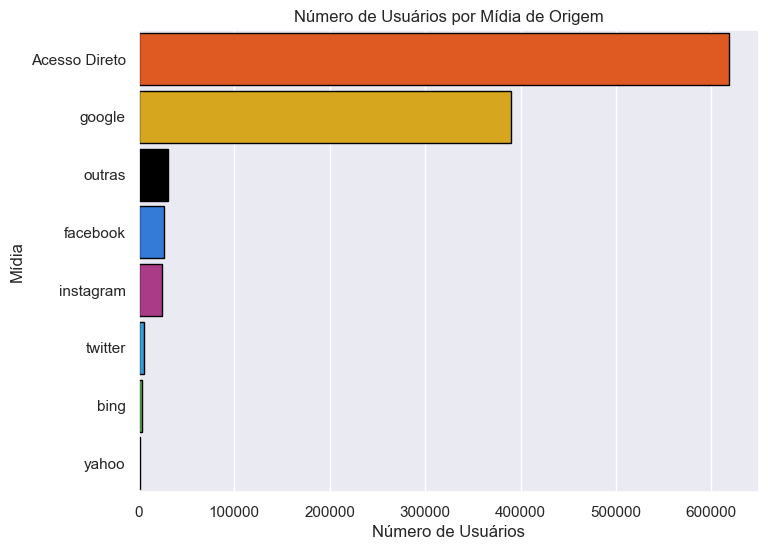
\includegraphics[width=1\textwidth]{C:/Users/Usuario/Desktop/Nova pasta/origem.png}%
\end{figure}

%
\newpage%
\subsection*{}%
\label{subsec:}%
Portal: 10 notícias mais vistas%


\begin{figure}[H]%
\centering%
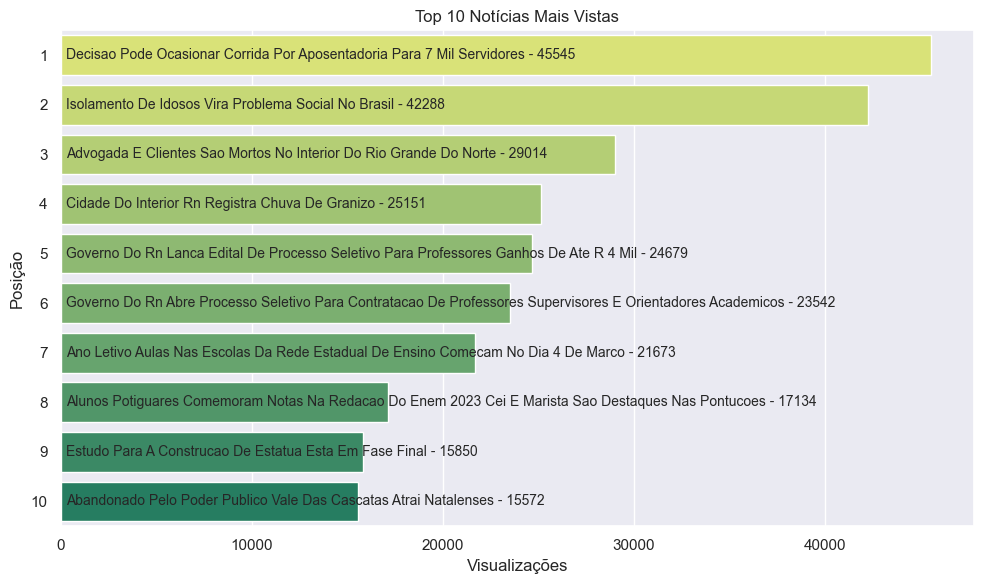
\includegraphics[width=0.8\textwidth]{C:/Users/Usuario/Desktop/Nova pasta/top10.png}%
\end{figure}

%
\subsection*{}%
\label{subsec:}%
Portal: 15 notícias mais pesquisadas%


\begin{figure}[H]%
\centering%
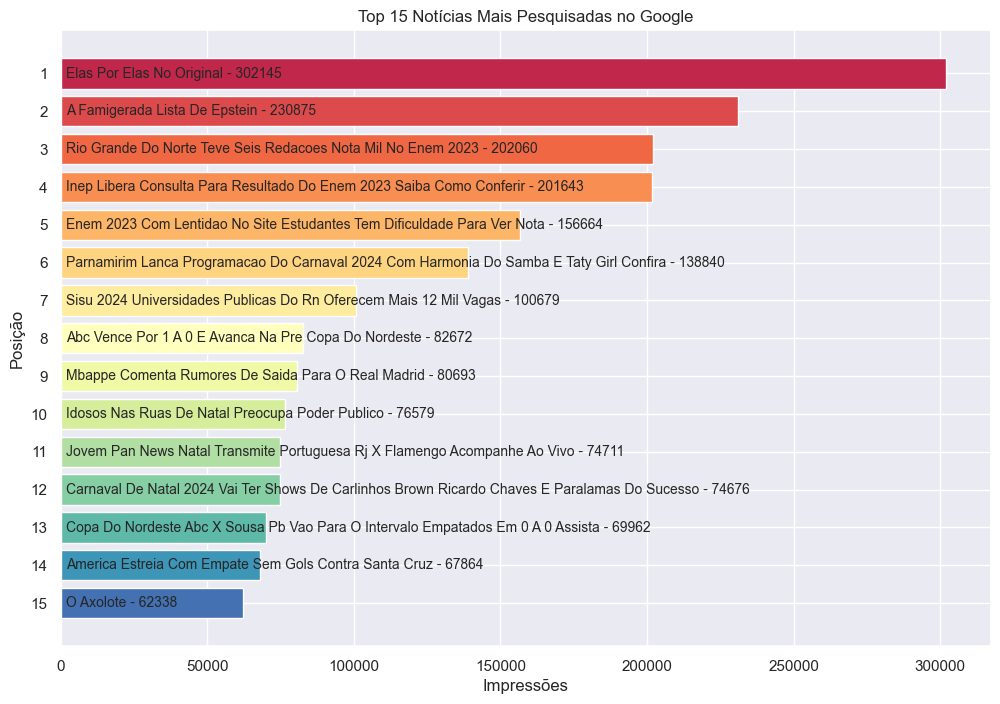
\includegraphics[width=0.9\textwidth]{C:/Users/Usuario/Desktop/Nova pasta/top15.png}%
\end{figure}

%
\subsection*{}%
\label{subsec:}%
Portal: comparativo de visualizações e acessos de usuários%


\begin{figure}[H]%
\centering%
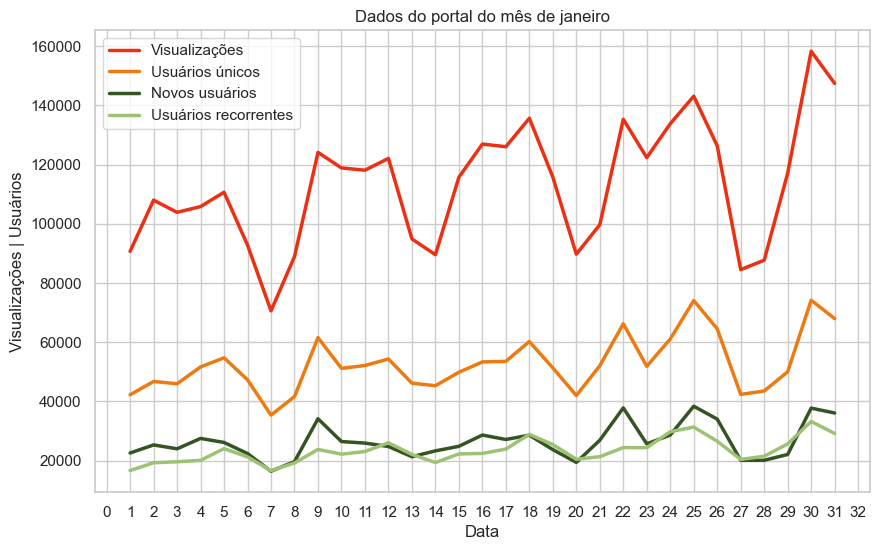
\includegraphics[width=0.8\textwidth]{C:/Users/Usuario/Desktop/Nova pasta/visualizacoesUsuarios.png}%
\end{figure}

%
\subsection*{}%
\label{subsec:}%
Portal: visualizações por faixa etária%


\begin{figure}[H]%
\centering%
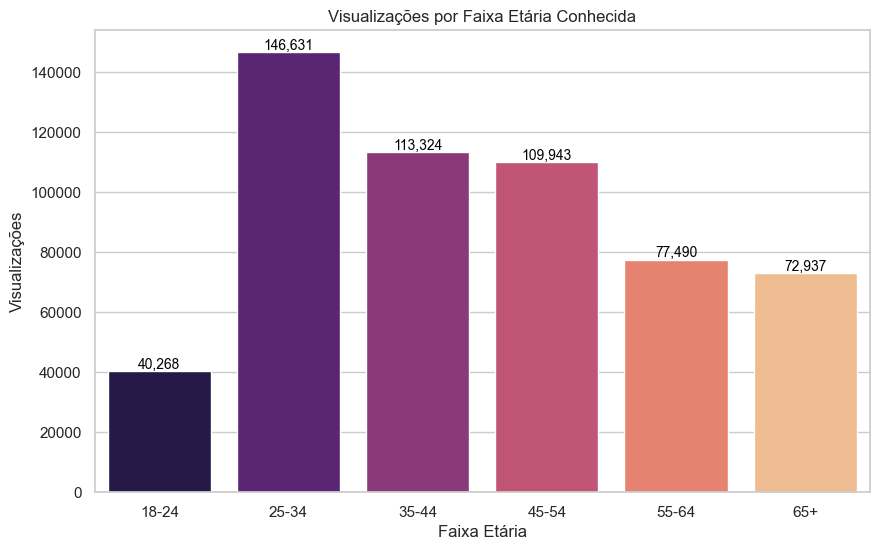
\includegraphics[width=0.8\textwidth]{C:/Users/Usuario/Desktop/Nova pasta/faixaEtaria.png}%
\end{figure}

%
\newpage%
\section*{}%
\label{sec:}%
Portal: visualizações por faixa etária (desconhecida e total)%


\begin{figure}[H]%
\centering%
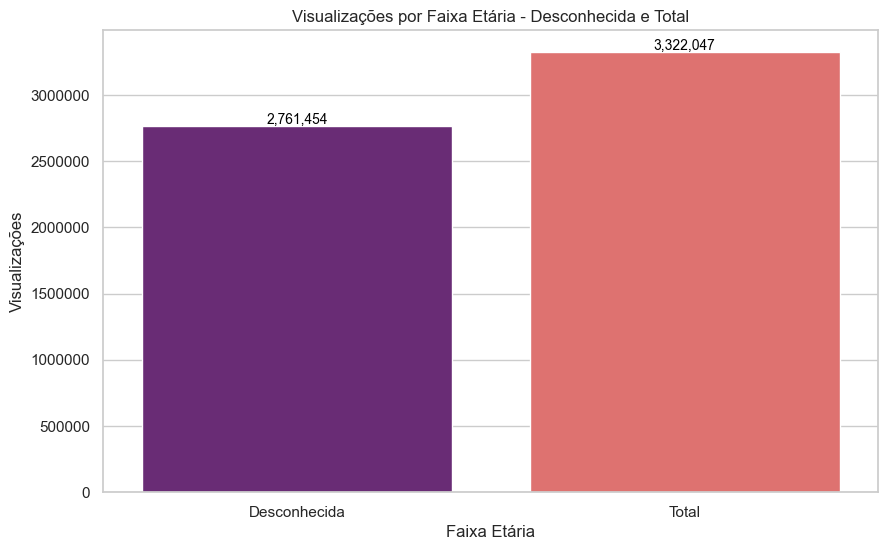
\includegraphics[width=0.8\textwidth]{C:/Users/Usuario/Desktop/Nova pasta/faixaEtaria_desconhecidaAndTotal.png}%
\end{figure}

%
\newpage%
\subsection*{Análise mensal}%
\label{subsec:Anlisemensal}%
\subsubsection*{Instagram}%
\label{ssubsec:Instagram}%
\begin{minipage}{\textwidth}%
\centering%
\begin{tabular}{@{}|c|c|c|c|@{}}%
\toprule%
\multirow{3}{*}{Mês}&Novos seguidores&Alcance&Visitas\\%
&\begin{footnotesize}%
variação em relação ao%
\end{footnotesize}&\begin{footnotesize}%
variação em relação ao%
\end{footnotesize}&\begin{footnotesize}%
variação em relação ao%
\end{footnotesize}\\%
&\begin{footnotesize}%
mês anterior | mesmo mês em 2023%
\end{footnotesize}&\begin{footnotesize}%
mês anterior | mesmo mês em 2023%
\end{footnotesize}&\begin{footnotesize}%
mês anterior | mesmo mês em 2023%
\end{footnotesize}\\%
\midrule%
\multirow{2}{*}{Janeiro}&6,7 mil&542 mil&152 mil\\%
&\begin{footnotesize}%
+21,8\% | +440,3\%%
\end{footnotesize}&\begin{footnotesize}%
{-}7\% | {-}19\%%
\end{footnotesize}&\begin{footnotesize}%
+17,2\% | {-}26,2\%%
\end{footnotesize}\\%
\midrule%
\multirow{2}{*}{Fevereiro}&5,8 mil&658,9 mil&144,7 mil\\%
&\begin{footnotesize}%
{-}16,09\% | {-}32,69\%%
\end{footnotesize}&\begin{footnotesize}%
+21,56\% | +2,53\%%
\end{footnotesize}&\begin{footnotesize}%
{-}4,7\% | {-}40,96\%%
\end{footnotesize}\\\bottomrule%
%
\end{tabular}%
\end{minipage}%
\begin{itemize}%
\item%
Legenda:%
\begin{enumerate}[label=-]%
\item%
\textbf{Alcance:} Essa métrica calcula o alcance da distribuição orgânica ou paga do seu conteúdo do Instagram e/ou Facebook, incluindo publicações e stories que foram turbinados. Também pode ser interpretada como a quantidade de contas atingidas;%
\item%
\textbf{Visitas:} número de vezes que usuários visitaram seu perfil.%
\end{enumerate}%
\end{itemize}

%
\subsection*{Análise mensal}%
\label{subsec:Anlisemensal}%
\subsubsection*{Facebook}%
\label{ssubsec:Facebook}%
\begin{minipage}{\textwidth}%
\centering%
\begin{tabular}{@{}|c|c|c|c|@{}}%
\toprule%
\multirow{3}{*}{Mês}&Novos seguidores&Alcance&Visitas\\%
&\begin{footnotesize}%
variação em relação ao%
\end{footnotesize}&\begin{footnotesize}%
variação em relação ao%
\end{footnotesize}&\begin{footnotesize}%
variação em relação ao%
\end{footnotesize}\\%
&\begin{footnotesize}%
mês anterior | mesmo mês em 2023%
\end{footnotesize}&\begin{footnotesize}%
mês anterior | mesmo mês em 2023%
\end{footnotesize}&\begin{footnotesize}%
mês anterior | mesmo mês em 2023%
\end{footnotesize}\\%
\midrule%
\multirow{2}{*}{Janeiro}&628&468 mil&32 mil\\%
&\begin{footnotesize}%
+38\% | +20\%%
\end{footnotesize}&\begin{footnotesize}%
{-}5\% | {-}7,5\%%
\end{footnotesize}&\begin{footnotesize}%
+9,6\% | +4,2\%%
\end{footnotesize}\\%
\midrule%
\multirow{2}{*}{Fevereiro}&('389', 0) &390,0 mil&31,4 mil\\%
&\begin{footnotesize}%
{-}38,06\% | {-}2,99\%%
\end{footnotesize}&\begin{footnotesize}%
{-}93,28\% | {-}93,16\%%
\end{footnotesize}&\begin{footnotesize}%
{-}2,16\% | +28,8\%%
\end{footnotesize}\\\bottomrule%
%
\end{tabular}%
\end{minipage}%
\begin{itemize}%
\item%
Legenda:%
\begin{enumerate}[label=-]%
\item%
\textbf{Alcance:} Essa métrica calcula o alcance da distribuição orgânica ou paga do seu conteúdo do Instagram e/ou Facebook, incluindo publicações e stories que foram turbinados. Também pode ser interpretada como a quantidade de contas atingidas;%
\item%
\textbf{Visitas:} número de vezes que usuários visitaram seu perfil.%
\end{enumerate}%
\end{itemize}

%
\newpage%
\section*{}%
\label{sec:}%
FB e IG: audiência por sexo e faixa etária%


\begin{figure}[H]%
\centering%
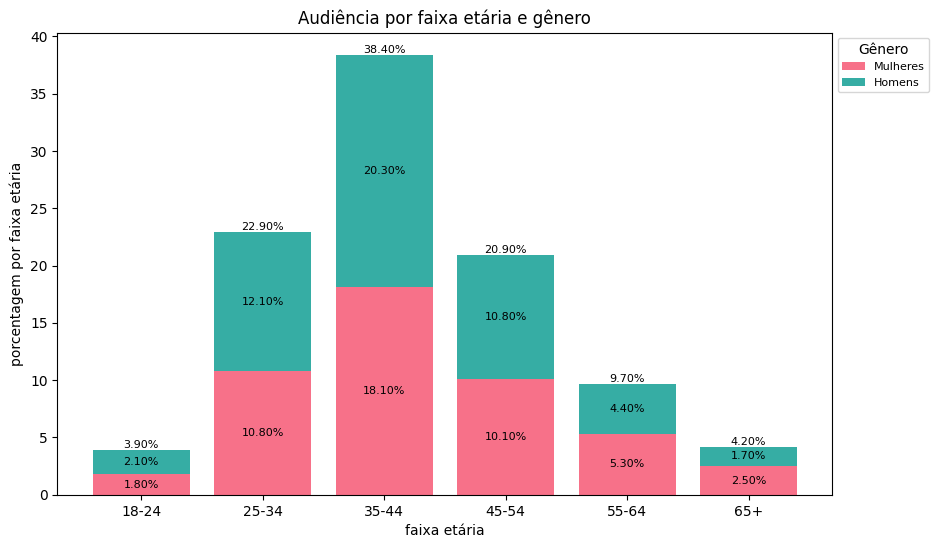
\includegraphics[width=0.8\textwidth]{C:/Users/Usuario/Desktop/Nova pasta/fePublico_FBIG.png}%
\end{figure}

%
\section*{}%
\label{sec:}%
FB e IG: audiência por cidades%


\begin{figure}[H]%
\centering%
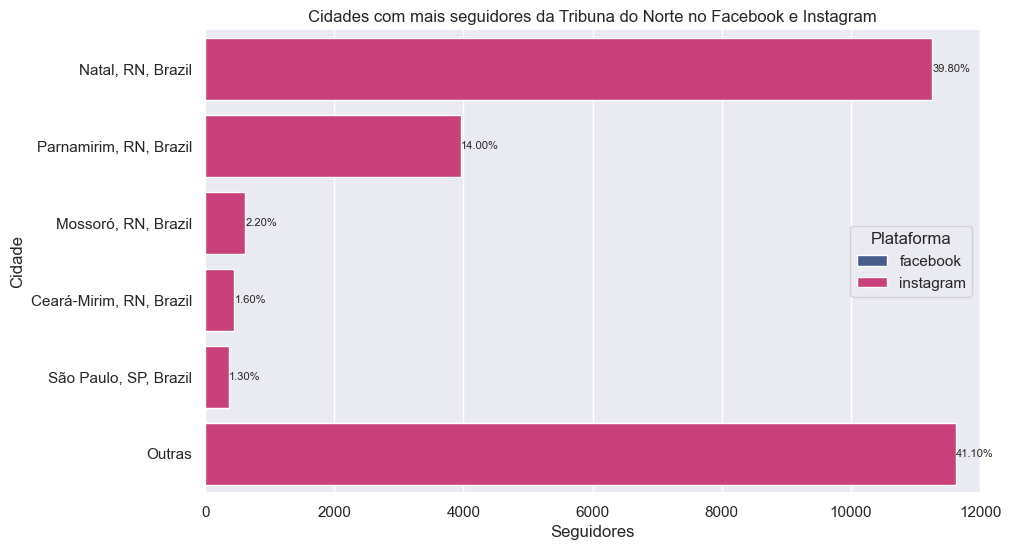
\includegraphics[width=0.8\textwidth]{C:/Users/Usuario/Desktop/Nova pasta/publicoCidades.png}%
\end{figure}

%
\newpage%
\section*{}%
\label{sec:}%
FB: visitas ao longo do mês%


\begin{figure}[H]%
\centering%
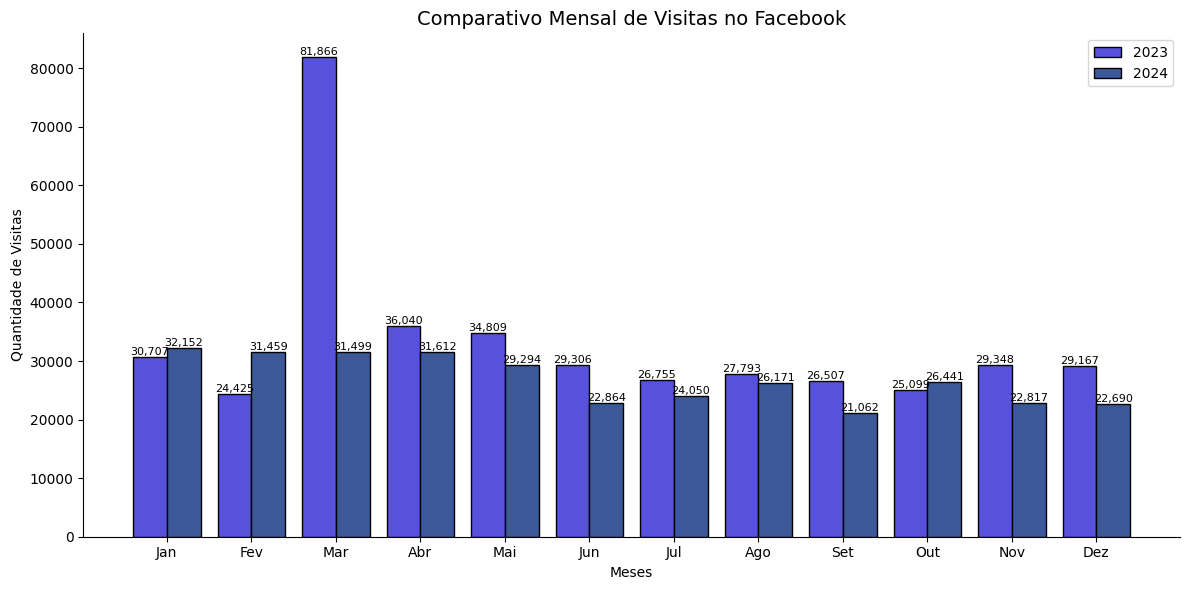
\includegraphics[width=0.75\textwidth]{C:/Users/Usuario/Desktop/Nova pasta/visitasFB.png}%
\end{figure}

%
\section*{}%
\label{sec:}%
FB: alcance ao longo do mês%


\begin{figure}[H]%
\centering%
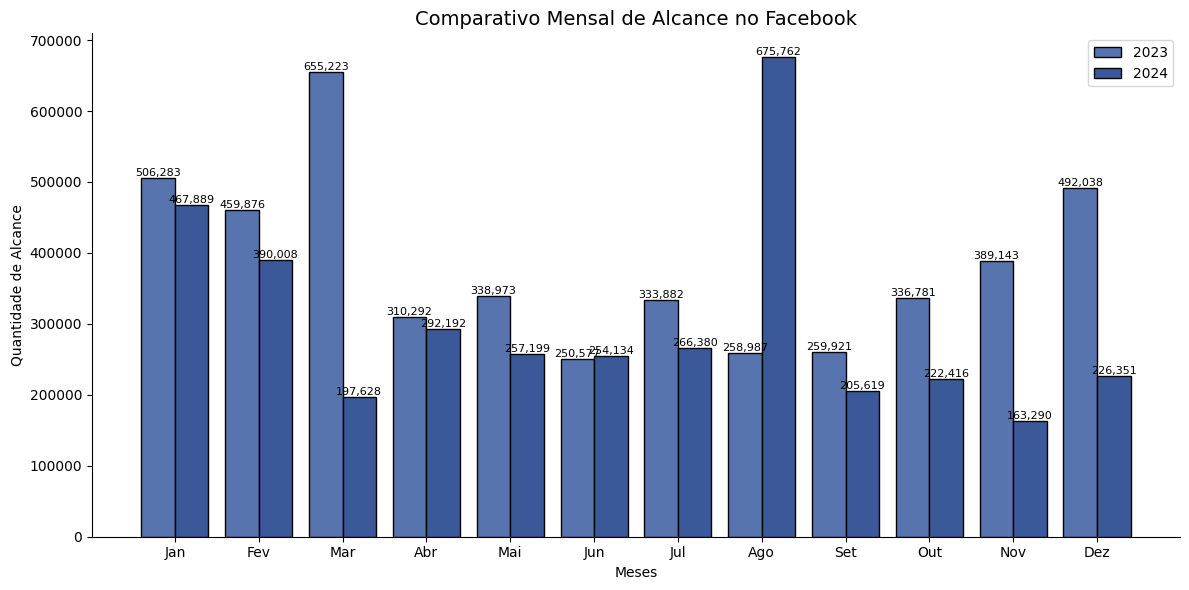
\includegraphics[width=0.75\textwidth]{C:/Users/Usuario/Desktop/Nova pasta/alcanceFB.png}%
\end{figure}

%
\section*{}%
\label{sec:}%
IG: ganho de seguidores ao longo do mês%


\begin{figure}[H]%
\centering%
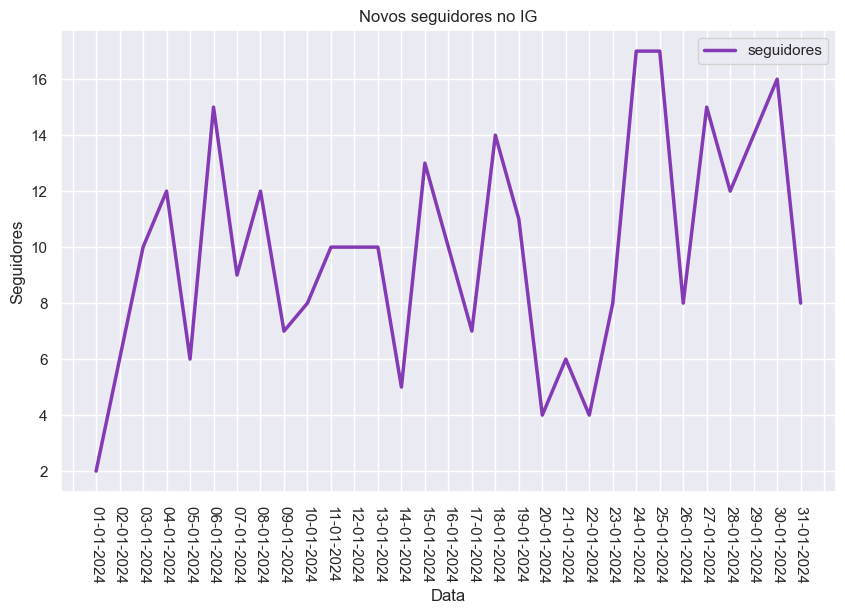
\includegraphics[width=0.45\textwidth]{C:/Users/Usuario/Desktop/Nova pasta/seguidoresIG.png}%
\end{figure}

%
\section*{}%
\label{sec:}%
IG: visitas ao perfil ao longo do mês%


\begin{figure}[H]%
\centering%
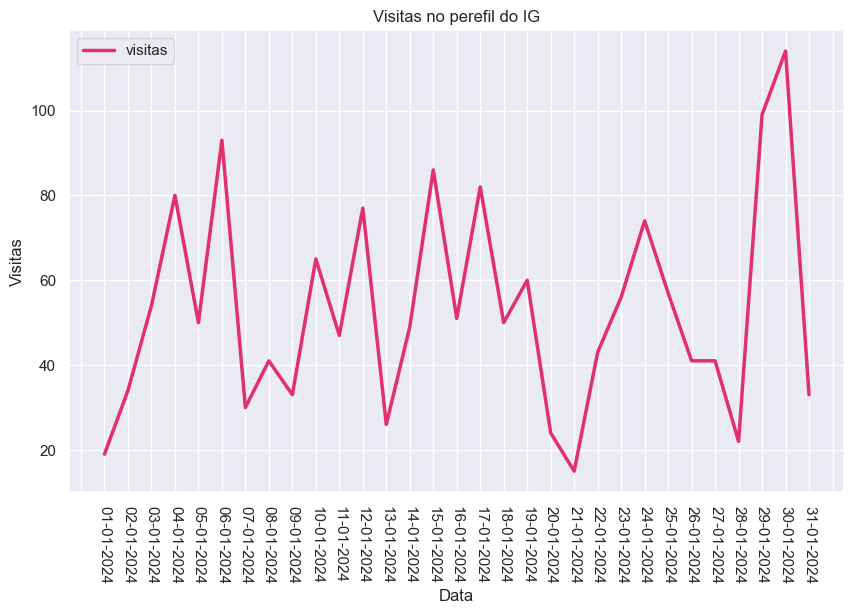
\includegraphics[width=0.45\textwidth]{C:/Users/Usuario/Desktop/Nova pasta/visitasIG.png}%
\end{figure}

%
\section*{}%
\label{sec:}%
IG: alcance do perfil ao longo do mês%


\begin{figure}[H]%
\centering%
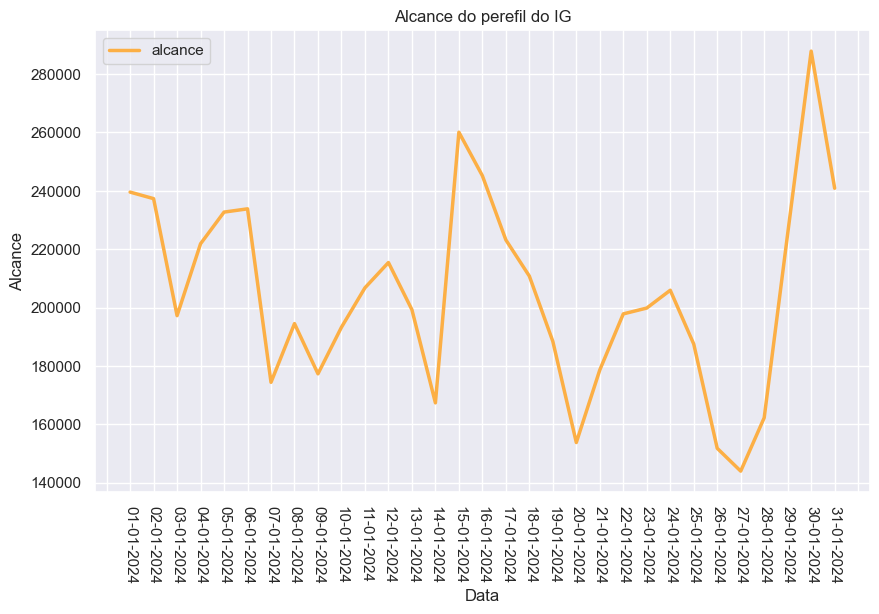
\includegraphics[width=0.45\textwidth]{C:/Users/Usuario/Desktop/Nova pasta/alcanceIG.png}%
\end{figure}

%
\newpage%
\section*{}%
\label{sec:}%
IG: comparativo de seguidores, visitas e alcance. (Obs.: dados fora de escala para uma melhor visualização)%


\begin{figure}[H]%
\centering%
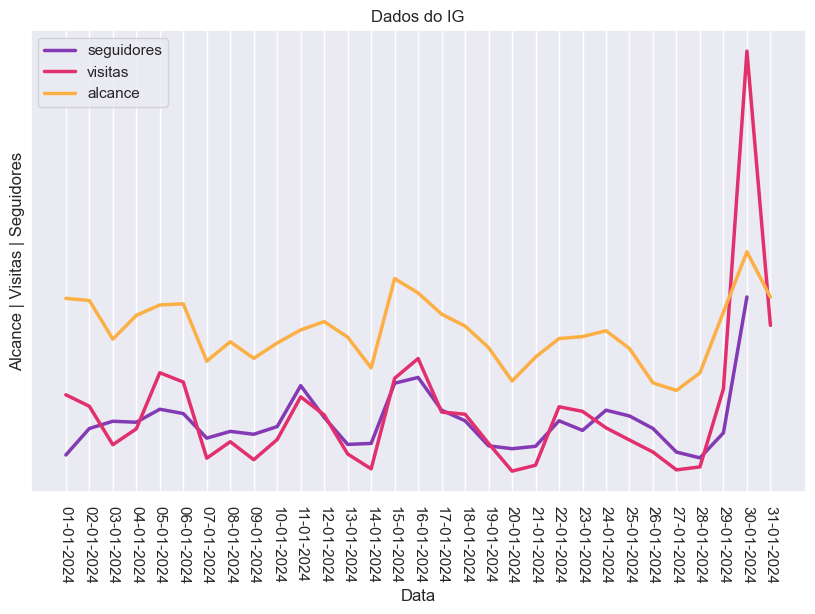
\includegraphics[width=1\textwidth]{C:/Users/Usuario/Desktop/Nova pasta/dadosIG.png}%
\end{figure}

%
\newpage%
\subsection*{Análise mensal}%
\label{subsec:Anlisemensal}%
\subsubsection*{Twitter}%
\label{ssubsec:Twitter}%
\begin{minipage}{\textwidth}%
\centering%
\begin{tabular}{@{}|c|c|c|c|@{}}%
\toprule%
\multirow{3}{*}{Mês}&Novos seguidores&Impressões&Engajamentos\\%
&\begin{footnotesize}%
variação em relação ao%
\end{footnotesize}&\begin{footnotesize}%
variação em relação ao%
\end{footnotesize}&\begin{footnotesize}%
variação em relação ao%
\end{footnotesize}\\%
&\begin{footnotesize}%
mês anterior | mesmo mês em 2023%
\end{footnotesize}&\begin{footnotesize}%
mês anterior | mesmo mês em 2023%
\end{footnotesize}&\begin{footnotesize}%
mês anterior | mesmo mês em 2023%
\end{footnotesize}\\%
\midrule%
\multirow{2}{*}{Janeiro}&2,9 mil&455,8 mil&13,2 mil\\%
&\begin{footnotesize}%
+81,3\% | +75,8\%%
\end{footnotesize}&\begin{footnotesize}%
+6\% | {-}59\%%
\end{footnotesize}&\begin{footnotesize}%
+22,2\% | {-}26,7\%%
\end{footnotesize}\\%
\midrule%
\multirow{2}{*}{Fevereiro}&2,0 mil&421,3 mil&11,2 mil\\%
&\begin{footnotesize}%
{-}30,17\% | +131,98\%%
\end{footnotesize}&\begin{footnotesize}%
{-}7,57\% | {-}27,16\%%
\end{footnotesize}&\begin{footnotesize}%
{-}14,89\% | +1,21\%%
\end{footnotesize}\\\bottomrule%
%
\end{tabular}%
\end{minipage}%
\begin{itemize}%
\item%
Legenda:%
\begin{enumerate}[label=-]%
\item%
\textbf{Impressões:} número de vezes que os usuários viram o(s) Tweet(s);%
\item%
\textbf{Engajamentos:} número total de vezes que um usuário interagiu com o(s) Tweet(s). Isso inclui todos os cliques em qualquer lugar no Tweet como: hashtags, links, avatar, nome de usuário e expansão do Tweet, Retweets, respostas e favoritos.%
\end{enumerate}%
\end{itemize}

%
\newpage%
\section*{}%
\label{sec:}%
TW: engajamento do twitter%


\begin{figure}[H]%
\centering%
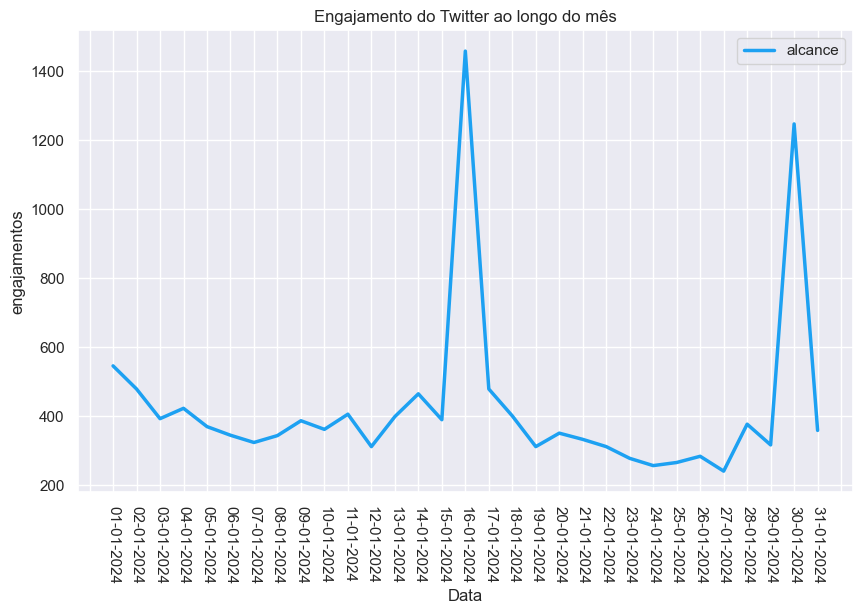
\includegraphics[width=0.45\textwidth]{C:/Users/Usuario/Desktop/Nova pasta/engajamentoTW.png}%
\end{figure}

%
\section*{}%
\label{sec:}%
TW: impressões do twitter%


\begin{figure}[H]%
\centering%
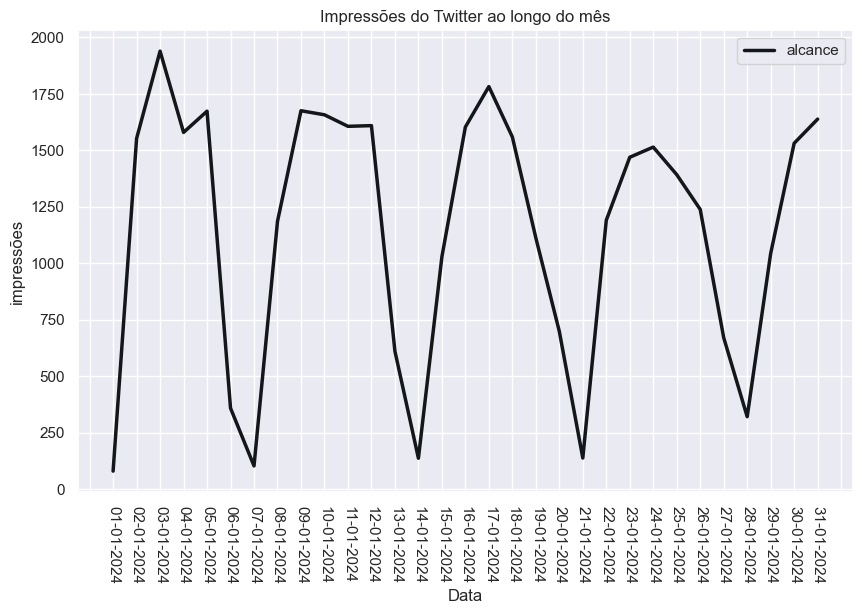
\includegraphics[width=0.45\textwidth]{C:/Users/Usuario/Desktop/Nova pasta/impressoesTW.png}%
\end{figure}

%
\section*{}%
\label{sec:}%
TW: ganho de seguidores no twitter ao logo do mês. (Esses dados levam em consideração apenas os ganhos)%


\begin{figure}[H]%
\centering%
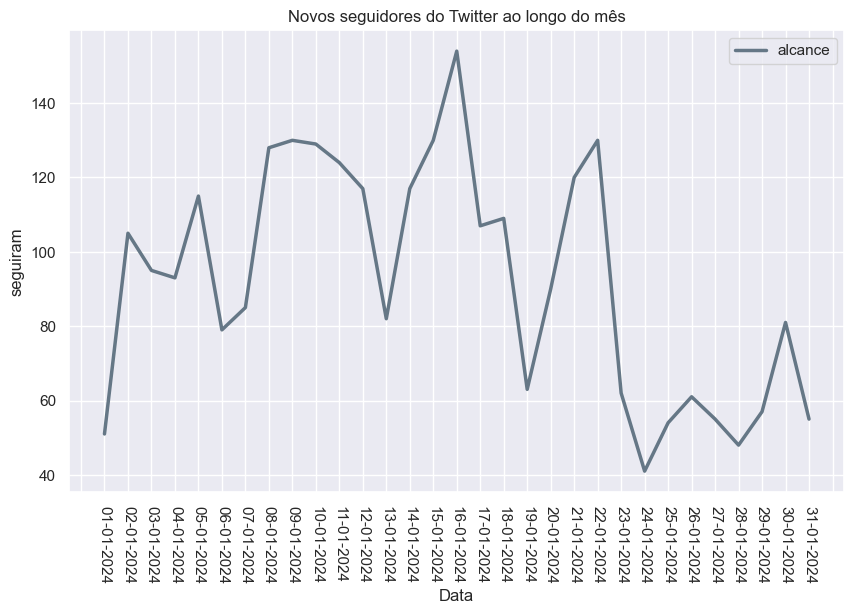
\includegraphics[width=0.45\textwidth]{C:/Users/Usuario/Desktop/Nova pasta/seguidoresTW.png}%
\end{figure}

%
\newpage%
\subsection*{Análise mensal}%
\label{subsec:Anlisemensal}%
\subsubsection*{YouTube}%
\label{ssubsec:YouTube}%
\begin{minipage}{\textwidth}%
\centering%
\begin{tabular}{@{}|c|c|c|c|@{}}%
\toprule%
\multirow{3}{*}{Mês}&Novos inscritos&Visualizações&Horas de exibição\\%
&\begin{footnotesize}%
variação em relação ao%
\end{footnotesize}&\begin{footnotesize}%
variação em relação ao%
\end{footnotesize}&\begin{footnotesize}%
variação em relação ao%
\end{footnotesize}\\%
&\begin{footnotesize}%
mês anterior | mesmo mês em 2023%
\end{footnotesize}&\begin{footnotesize}%
mês anterior | mesmo mês em 2023%
\end{footnotesize}&\begin{footnotesize}%
mês anterior | mesmo mês em 2023%
\end{footnotesize}\\%
\midrule%
\multirow{2}{*}{Janeiro}&484&132 mil&2,3 mil\\%
&\begin{footnotesize}%
+95,2\% | +389\%%
\end{footnotesize}&\begin{footnotesize}%
+95,3\% | +288\%%
\end{footnotesize}&\begin{footnotesize}%
+48\% | +172,2\%%
\end{footnotesize}\\%
\midrule%
\multirow{2}{*}{Fevereiro}&('614', 0) &137,3 mil&4,2 mil\\%
&\begin{footnotesize}%
+47,95\% | +176,58\%%
\end{footnotesize}&\begin{footnotesize}%
+3,73\% | +89,65\%%
\end{footnotesize}&\begin{footnotesize}%
+79,31\% | +196,31\%%
\end{footnotesize}\\\bottomrule%
%
\end{tabular}%
\end{minipage}

%
\section*{}%
\label{sec:}%
YouTube: visualizações por faixa etári a%


\begin{figure}[H]%
\centering%
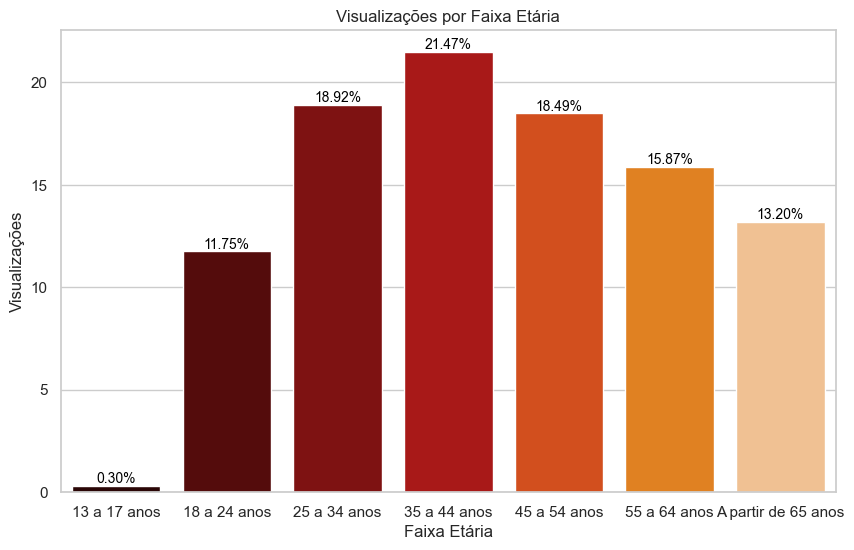
\includegraphics[width=0.7\textwidth]{C:/Users/Usuario/Desktop/Nova pasta/visualizacoesIdadeYTB.png}%
\end{figure}

%
\newpage%
\section*{}%
\label{sec:}%
YouTube: horas de exibição por faixa etária%


\begin{figure}[H]%
\centering%
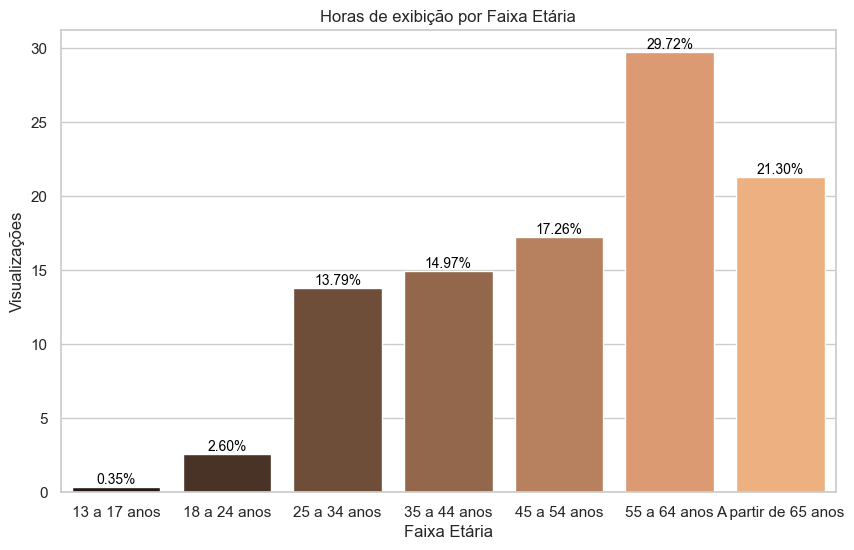
\includegraphics[width=0.7\textwidth]{C:/Users/Usuario/Desktop/Nova pasta/horasIdadeYTB.png}%
\end{figure}

%
\section*{}%
\label{sec:}%
YouTube: sexo do público%


\begin{figure}[H]%
\centering%
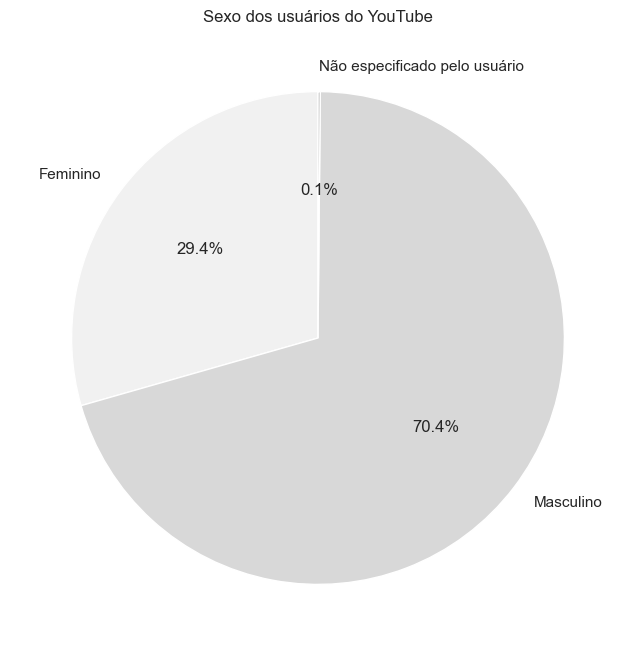
\includegraphics[width=0.6\textwidth]{C:/Users/Usuario/Desktop/Nova pasta/generoYTB.png}%
\end{figure}

%
\section*{}%
\label{sec:}%
YouTube: visualizações por cidade%


\begin{figure}[H]%
\centering%
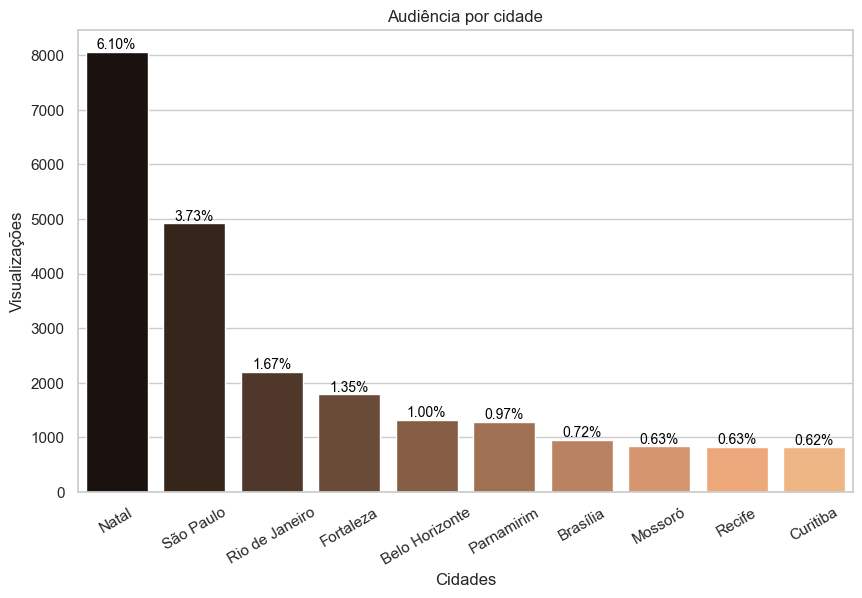
\includegraphics[width=0.7\textwidth]{C:/Users/Usuario/Desktop/Nova pasta/visualizacoesCidadeYTB.png}%
\end{figure}

%
\newpage%
\begin{itemize}%
\item%
Funcionamento dos algoritmos:%
\begin{enumerate}[label=-]%
\item%
\textbf{Facebook:} O algoritmo do Facebook prioriza os conteúdos que geram mais interações, como curtidas, comentários e compartilhamentos. Ele também considera o grau de relacionamento entre os usuários e as contas que eles seguem, mostrando mais publicações de amigos e familiares do que de páginas. Além disso, o Facebook leva em conta a relevância e a atualidade dos conteúdos, dando mais destaque para as notícias e os assuntos do momento;%
\item%
\textbf{Instagram:} O a lgoritmo do Instagram também se baseia no engajamento, no relacionamento e na temporalidade dos conteúdos. Ele mostra primeiro as postagens e as histórias das contas com as quais o usuário mais interage, seja por meio de curtidas, comentários, mensagens diretas ou buscas. Ele também valoriza os conteúdos mais recentes e mais relevantes para o usuário, de acordo com os seus interesses e hábitos;%
\item%
\textbf{Twitter:} O algoritmo do Twitter tem duas formas de exibir os conteúdos: o modo cronológico e o modo destacado. No modo cronológico, o usuário vê os tweets mais recentes em ordem de publicação. No modo destacado, o usuário vê os tweets mais relevantes para ele, de acordo com o seu perfil, as suas interações e os assuntos do momento. O Twitter também mostra os tweets mais populares e mais comentados na seção “O que está acontecendo”;%
\item%
\textbf{YouTube:} O algoritmo do YouTube tem como objetivo aumentar o tempo de permanência dos usuários na plataforma, recomendando os vídeos que eles têm mais chances de assistir e se engajar. Para isso, ele considera fatores como o histórico de visualização, as preferências, as inscrições, a localização e o feedback dos usuários. Ele também leva em conta a qualidade e a relevância dos vídeos, analisando aspectos como o título, descrição, tags, miniaturas e os metadados.%
\end{enumerate}%
\end{itemize}%
\end{document}